In each of the following exercises, find the coordinates of the foci, the vertices,the length of major axis, the minor axis,the eccentricity and the length of the latus rectum of the ellipse.
\begin{enumerate}[label=\thesection.\arabic*,ref=\thesection.\theenumi]
\numberwithin{equation}{enumi}
\numberwithin{figure}{enumi}
\numberwithin{table}{enumi}


  \item $\frac{x^2}{36}+\frac{y^2}{16}=1$
  \item $\frac{x^2}{4}+\frac{y^2}{25}=1$
\\
\solution
\iffalse
\documentclass[12pt]{article}
\usepackage{graphicx}
\usepackage{amsmath}
\usepackage{mathtools}
\usepackage{gensymb}

\newcommand{\mydet}[1]{\ensuremath{\begin{vmatrix}#1\end{vmatrix}}}
\providecommand{\brak}[1]{\ensuremath{\left(#1\right)}}
\providecommand{\norm}[1]{\left\lVert#1\right\rVert}
\providecommand{\abs}[1]{\left\vert#1\right\vert}
\newcommand{\solution}{\noindent \textbf{Solution: }}
\newcommand{\myvec}[1]{\ensuremath{\begin{pmatrix}#1\end{pmatrix}}}
\let\vec\mathbf

\begin{document}
\begin{center}
\textbf\large{CONIC SECTIONS}

\end{center}
\section*{Excercise 11.3}
Q2.Find the coordinates of the focii, the vertices, the length of major and minor axes, the eccentricity and the length of the latus rectum of an ellipse whose equation is given by $\frac{x^2}{4}+\frac{y^2}{25}=1$.

\solution
\fi
The equation of the given ellipse can be rearranged as 
\begin{align}
	\label{eq:chapters/11/11/3/2/eq1}
	25x^2+4y^2-100=0
\end{align}
The above equation can be equated to the generic equation of conic sections
\begin{align}
	\label{eq:chapters/11/11/3/2/eq2}
	g\brak{\vec{x}}=\vec{x}^\top \vec{V} \vec{x} + 2\vec{u}^\top \vec{x} + f = 0
\end{align}
Comparing coefficients of both equations \eqref{eq:chapters/11/11/3/2/eq1} and \eqref{eq:chapters/11/11/3/2/eq2}
\begin{align}
	\label{eq:chapters/11/11/3/2/eq3}
	\vec{V} &= \myvec{25&0\\0&4}\\
	\vec{u} &= \vec{0}\\
	f &= -100
\end{align}
From equation \eqref{eq:chapters/11/11/3/2/eq3}, since $\vec{V}$ is already diagonalized, the eigen values $\lambda_1 \text{ and } \lambda_2$ are given as
\begin{align}
	\lambda_1 &= 25\\
	\lambda_2 &= 4
\end{align}
Since the given matrix $\vec{V}$ is diagonal, the Eigen vector matrix will be identity. It is given as
\begin{align}
	\vec{P} &= \myvec{\vec{p}_1 & \vec{p}_2}\\
		&= \myvec{1&0\\0&1}
\end{align}
\begin{enumerate}
\item The eccentricity of the ellipse is given as
\begin{align}
	e &= \sqrt{1 - \frac{\lambda_2}{\lambda_1}} = \sqrt{1-\frac{4}{25}}\\
	  &= \frac{\sqrt{21}}{5}
\end{align}
\item Finding the coordinates of Focii
\begin{align}
	\vec{n} &= \sqrt{\lambda_1}\vec{p}_2= \sqrt{25} \myvec{0\\1}\\
	&= \myvec{0\\5}
\end{align}
\begin{align}
	\label{eq:chapters/11/11/3/2/eq4}
	c &= \frac{e\vec{u}^\top \vec{n} \pm \sqrt{e^2 \brak{\vec{u}^\top \vec{n}}^2-\lambda_1 \brak{e^2 -1}\brak{\norm{\vec{u}}^2-\lambda_1 f}}}{\lambda_1 e\brak{e^2-1}}
\end{align}
Substituting values of $e,\vec{u},\vec{n},\lambda_1 \text{ and } f$ in \eqref{eq:chapters/11/11/3/2/eq4}
\begin{align}
	c &= \frac{0 \pm \sqrt{0-25\brak{\frac{21}{25}-1}\brak{0+25\brak{100}}}}{25\frac{\sqrt{21}}{5}\brak{\frac{21}{25}-1}}\\
	&= \frac{\pm 125}{\sqrt{21}}
\end{align}
The focus $\vec{F}$ of the ellipse is expressed as
\begin{align}
	\vec{F} &= \frac{ce^2 \vec{n}-\vec{u}}{\lambda_1}\\
	&= \frac{\pm \frac{125}{\sqrt{21}}\brak{\frac{21}{25}}\myvec{0\\5}}{25}\\
	&= \myvec{0\\\pm \sqrt{21}}
\end{align}
\item The length of the major axis is given by
\begin{align}
	\label{eq:chapters/11/11/3/2/eq5}
	&2\sqrt{\abs{\frac{f_0}{\lambda_2}}}\\
	f_0 &= \vec{u}^\top \vec{V}^{-1} \vec{u} -f\\
	    &= 100\\
	\eqref{eq:chapters/11/11/3/2/eq5} &\implies 2\sqrt{\abs{\frac{100}{4}}}
	 = 10
\end{align}
\item The length of minor axis is given by
\begin{align}
	2\sqrt{\abs{\frac{f_0}{\lambda_1}}}&= 2\sqrt{\abs{\frac{100}{25}}}\\
	&= 4
\end{align}
\item The vertices of the ellipse are given by
\begin{align}
	\pm \myvec{0\\\sqrt{\abs{\frac{f_0}{\lambda_2}}}}= \pm \myvec{0\\5}
\end{align}
\item The length of latus rectum is given as
\begin{align}
	2\frac{\sqrt{\abs{f_0 \lambda_2}}}{\lambda_1} &= 2\frac{\sqrt{\abs{100\brak{4}}}}{25}\\
	&= \frac{8}{5}
\end{align}
\end{enumerate}
The corresponding is shown in Fig. \ref{fig:chapters/11/11/3/2/Fig1}.
\begin{figure}[!h]
	\begin{center} 
	    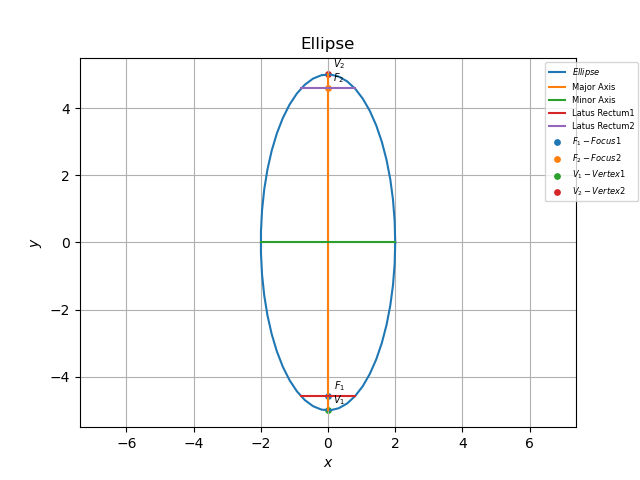
\includegraphics[width=\columnwidth]{chapters/11/11/3/2/figs/ellipse}
	\end{center}
\caption{}
\label{fig:chapters/11/11/3/2/Fig1}
\end{figure}

  \item $\frac{x^2}{16}+\frac{y^2}{9}=1$
  \item $\frac{x^2}{25}+\frac{y^2}{100}=1$
  \item $\frac{x^2}{49}+\frac{y^2}{36}=1$
  \item $\frac{x^2}{100}+\frac{y^2}{400}=1$
  \item $36x^2+4y^2=144$
  \item $16x^2+y^2=16$
  \item $4x^2+9y^2=36$
\end{enumerate}

In each of the following exercises,  find the equation for the ellipse that satisfies the given conditions

%\begin{enumerate}[label=\thesection.\arabic*,ref=\thesection.\theenumi][resume]
\begin{enumerate}[resume*]
\item vertices $(\pm5,0),\text{foci} (\pm4,0)$
\item vertices $(\pm0,13),\text{foci} (0,\pm5)$
\item vertices $(\pm6,0),\text{foci} (\pm4,0)$
\item Ends of major axis $(\pm3,0),\text{ends of minor axis}(0,\pm2)$
\item  ends of major axis $(0,\pm \sqrt{5}),\text{ends of minor axis} (\pm1,0)$
\item $\text {length of major axis 26},\text{foci} (\pm5,0)$
\item $\text {length of minor axis 16},\text{foci} (0,\pm6)$
\item $\text {foci} (\pm3,0),a=4$
\item $\text {b=3,c=4},\text {centre at the origin} ;\text{foci on the x axis}$
\item $\text {centre at} (0,0),\text{major axis on the y-axis and passes through the points} \text {(3,2) and (1,6)}$
\item $\text{major axis on the x-axis and passes through the points (4,3) and (6,2)}$
\\
\solution
\iffalse
\documentclass[journal,12pt,twocolumn]{IEEEtran}
\usepackage{setspace}
\usepackage{gensymb}
\usepackage{xcolor}
\usepackage{caption}
\singlespacing
\usepackage{siunitx}
\usepackage[cmex10]{amsmath}
\usepackage{mathtools}
\usepackage{hyperref}
\usepackage{amsthm}
\usepackage{mathrsfs}
\usepackage{txfonts}
\usepackage{stfloats}
\usepackage{cite}
\usepackage{cases}
\usepackage{subfig}
\usepackage{longtable}
\usepackage{multirow}
\usepackage{enumitem}
\usepackage{bm}
\usepackage{mathtools}
\usepackage{listings}
\usepackage{tikz}
\usetikzlibrary{shapes,arrows,positioning}
\usepackage{circuitikz}
\renewcommand{\vec}[1]{\boldsymbol{\mathbf{#1}}}
\DeclareMathOperator*{\Res}{Res}
\renewcommand\thesection{\arabic{section}}
\renewcommand\thesubsection{\thesection.\arabic{subsection}}
\renewcommand\thesubsubsection{\thesubsection.\arabic{subsubsection}}

\renewcommand\thesectiondis{\arabic{section}}
\renewcommand\thesubsectiondis{\thesectiondis.\arabic{subsection}}
\renewcommand\thesubsubsectiondis{\thesubsectiondis.\arabic{subsubsection}}
\hyphenation{op-tical net-works semi-conduc-tor}

\lstset{
language=Python,
frame=single, 
breaklines=true,
columns=fullflexible
}
\begin{document}
\theoremstyle{definition}
\newtheorem{theorem}{Theorem}[section]
\newtheorem{problem}{Problem}
\newtheorem{proposition}{Proposition}[section]
\newtheorem{lemma}{Lemma}[section]
\newtheorem{corollary}[theorem]{Corollary}
\newtheorem{example}{Example}[section]
\newtheorem{definition}{Definition}[section]
\newcommand{\BEQA}{\begin{eqnarray}}
\newcommand{\EEQA}{\end{eqnarray}}
\newcommand{\define}{\stackrel{\triangle}{=}}
\newcommand{\myvec}[1]{\ensuremath{\begin{pmatrix}#1\end{pmatrix}}}
\newcommand{\mydet}[1]{\ensuremath{\begin{vmatrix}#1\end{vmatrix}}}
\bibliographystyle{IEEEtran}
\providecommand{\nCr}[2]{\,^{#1}C_{#2}} % nCr
\providecommand{\nPr}[2]{\,^{#1}P_{#2}} % nPr
\providecommand{\mbf}{\mathbf}
\providecommand{\pr}[1]{\ensuremath{\Pr\left(#1\right)}}
\providecommand{\qfunc}[1]{\ensuremath{Q\left(#1\right)}}
\providecommand{\sbrak}[1]{\ensuremath{{}\left[#1\right]}}
\providecommand{\lsbrak}[1]{\ensuremath{{}\left[#1\right.}}
\providecommand{\rsbrak}[1]{\ensuremath{{}\left.#1\right]}}
\providecommand{\brak}[1]{\ensuremath{\left(#1\right)}}
\providecommand{\lbrak}[1]{\ensuremath{\left(#1\right.}}
\providecommand{\rbrak}[1]{\ensuremath{\left.#1\right)}}
\providecommand{\cbrak}[1]{\ensuremath{\left\{#1\right\}}}
\providecommand{\lcbrak}[1]{\ensuremath{\left\{#1\right.}}
\providecommand{\rcbrak}[1]{\ensuremath{\left.#1\right\}}}
\theoremstyle{remark}
\newtheorem{rem}{Remark}
\newcommand{\sgn}{\mathop{\mathrm{sgn}}}
\newcommand{\rect}{\mathop{\mathrm{rect}}}
\newcommand{\sinc}{\mathop{\mathrm{sinc}}}
\providecommand{\abs}[1]{\left\vert#1\right\vert}
\providecommand{\res}[1]{\Res\displaylimits_{#1}} 
\providecommand{\norm}[1]{\lVert#1\rVert}
\providecommand{\mtx}[1]{\mathbf{#1}}
\providecommand{\mean}[1]{E\left[ #1 \right]}
\providecommand{\fourier}{\overset{\mathcal{F}}{ \rightleftharpoons}}
\providecommand{\ztrans}{\overset{\mathcal{Z}}{ \rightleftharpoons}}
\providecommand{\system}[1]{\overset{\mathcal{#1}}{ \longleftrightarrow}}
\newcommand{\solution}{\noindent \textbf{Solution: }}
\providecommand{\dec}[2]{\ensuremath{\overset{#1}{\underset{#2}{\gtrless}}}}
\let\StandardTheFigure\thefigure
\def\putbox#1#2#3{\makebox[0in][l]{\makebox[#1][l]{}\raisebox{\baselineskip}[0in][0in]{\raisebox{#2}[0in][0in]{#3}}}}
     \def\rightbox#1{\makebox[0in][r]{#1}}
     \def\centbox#1{\makebox[0in]{#1}}
     \def\topbox#1{\raisebox{-\baselineskip}[0in][0in]{#1}}
     \def\midbox#1{\raisebox{-0.5\baselineskip}[0in][0in]{#1}}

\vspace{3cm}
\title{Conic Assignment}
\author{Gautam Singh}
\maketitle
\bigskip

\begin{abstract}
    This document contains the solution to Question 20 of Exercise 3 in Chapter
    11 of the class 11 NCERT textbook.
\end{abstract}

\begin{enumerate}
    \item Find the equation of the ellipse whose major axis is the $x$-axis and
    center is the origin and passes through the points
    \begin{align}
        \vec{P} = \myvec{4\\3},\ \vec{Q} = \myvec{6\\2}
    \end{align}

    \solution 
\fi
		Let the equation of the conic with focus $\vec{F}$, directrix
    $\vec{n}^\top\vec{x} = c$ and eccentricity $e$ be
    \begin{align}
        \vec{x}^\top\vec{V}\vec{x} + 2\vec{u}^\top\vec{x} + f = 0
        \label{eq:chapters/11/11/3/20/conic-def}
    \end{align}
    where
    \begin{align}
        \vec{V} &\triangleq \norm{\vec{n}}^2\vec{I} - e^2\vec{n}\vec{n}^\top \label{eq:chapters/11/11/3/20/V-def} \\
        \vec{u} &\triangleq ce^2\vec{n} - \norm{\vec{n}}^2\vec{F} \label{eq:chapters/11/11/3/20/u-def} \\
        f &\triangleq \norm{\vec{n}}^2\norm{\vec{F}}^2 - c^2e^2 \label{eq:chapters/11/11/3/20/f-def}
    \end{align}
    Since the conic is an ellipse whose major axis is along the $x$-axis, we have
    \begin{align}
        \vec{n} = \myvec{1\\0}
    \end{align}
    Thus,
    \begin{align}
        \vec{V} = \myvec{1-e^2&0\\0&1} \label{eq:chapters/11/11/3/20/V-val} \\
        \vec{u} = ce^2\myvec{1\\0} - \vec{F} \label{eq:chapters/11/11/3/20/u-val} \\
        f = \norm{\vec{F}}^2 - c^2e^2 \label{eq:chapters/11/11/3/20/f-val}
    \end{align}
    The centre of the conic is given by
    \begin{align}
        \vec{c} = -\vec{V}^{-1}\vec{u}
        \label{eq:chapters/11/11/3/20/center}
    \end{align}
    Since $\vec{c} = \vec{0}$ and $\vec{V}^{-1} \neq \vec{0}$, it follows from 
    \eqref{eq:chapters/11/11/3/20/center} that $\vec{u} = \vec{0}$. Thus, from \eqref{eq:chapters/11/11/3/20/u-val},
    \begin{align}
        \vec{F} = \myvec{ce^2\\0}
        \label{eq:chapters/11/11/3/20/F-c-e}
    \end{align}
    and so,
    \begin{align}
        f = c^2e^2\brak{e^2-1}
        \label{eq:chapters/11/11/3/20/f-c-e}
    \end{align}
    Putting $\vec{x} = \vec{P}$ in \eqref{eq:chapters/11/11/3/20/conic-def} and using \eqref{eq:chapters/11/11/3/20/F-c-e}
    and \eqref{eq:chapters/11/11/3/20/f-c-e},
    \begin{align}
        \myvec{4&3}\myvec{1-e^2&0\\0&1}\myvec{4\\3} + f &= 0 \\
        \implies 16e^2 - f = 25 \label{eq:chapters/11/11/3/20/e1}
    \end{align}
    Putting $\vec{x} = \vec{Q}$ in \eqref{eq:chapters/11/11/3/20/conic-def}, we get
    \begin{align}
        \myvec{6&2}\myvec{1-e^2&0\\0&1}\myvec{6\\2} + f &= 0 \\
        \implies 36e^2 - f = 40 \label{eq:chapters/11/11/3/20/e2}
    \end{align}
    The equations \eqref{eq:chapters/11/11/3/20/e1} and \eqref{eq:chapters/11/11/3/20/e2} can be formulated as
    a matrix equation
    \begin{align}
        \myvec{16&-1\\36&-1}\myvec{e^2\\f} = \myvec{25\\40}
        \label{eq:chapters/11/11/3/20/mtx-eqn}
    \end{align}
    and can be solved using the augmented matrix.
    \begin{align}
        \myvec{16&-1&25\\36&-1&40} &\xleftrightarrow[]{R_1\leftarrow R_1-R_2} \myvec{-20&0&-15\\36&-1&40} \\
                 &\xleftrightarrow[]{\substack{R_1\leftarrow\frac{R_1}{-5}\\R_2\leftarrow -R_2}} \myvec{4&0&3\\-36&1&-40} \\
                 &\xleftrightarrow[]{R_2\leftarrow R_2+9R_1}\myvec{4&0&3\\0&1&-13} \\
                 &\xleftrightarrow[]{R_1\leftarrow\frac{R_1}{4}}\myvec{1&0&\frac{3}{4}\\0&1&-13}
    \end{align}
    Thus,
    \begin{align}
        e^2 = \frac{3}{4},\ f = -13
    \end{align}
    And the equation of the conic is given by
    \begin{align}
        \vec{x}^\top\myvec{\frac{1}{4}&0\\0&1}\vec{x} - 13 = 0
    \end{align}
    The situation is illustrated in Fig. \ref{fig:chapters/11/11/3/20/ellipse}
    \begin{figure}[!ht]
        \centering
        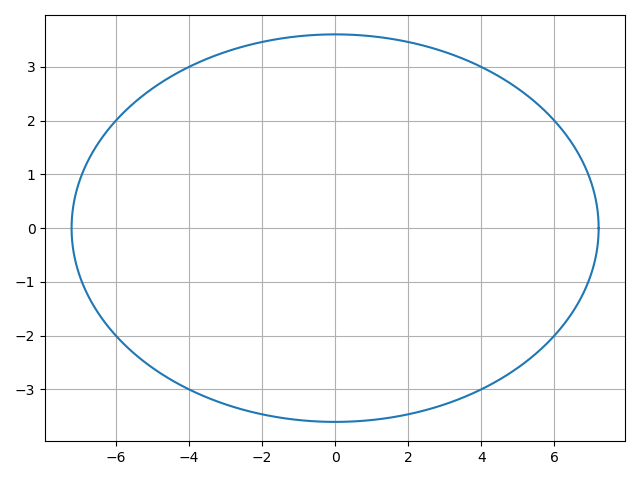
\includegraphics[width=\columnwidth]{chapters/11/11/3/20/figs/ellipse.png}
        \caption{Locus of the required ellipse.}
        \label{fig:chapters/11/11/3/20/ellipse}
    \end{figure}


\end{enumerate}
